\section{Obserwacje i wnioski}

\subsection{Zalety aplikacji}

Aplikacja pozwala na bieżąco monitorować stan powietrza w niektórych salach Politechniki Wrocławskiej. W trakcie pisania pracy są to
cztery czujniki rozmieszczone w czterech różnych salach budynku C2. Dzięki zapisowi do bazy danych możliwe jest badanie danych historycznych z dowolnych
przedziałów, co pozwala obserwować wpływ takich czynników jak liczebność studentów w sali czy pora roku na jakość powietrza w budynku.

Prowadzenie innych statystyk i praca z danymi jest również możliwa dzięki możliwości pobrania danych w formacie CSV. Czytelny interfejs pomaga w 
szybkiej ocenie przebiegu parametrów na przestrzeni dnia lub innego wybranego okresu

\subsection{Wady i rozwój}

W trakcie prac nad projektem wielokrotnie doświadczano trudności związanych z obsługą urządzeń wykorzystujących technologię IQRF. Czujniki zdawały się
być bardzo "wrażliwe" na jakiekolwiek zmiany w ich otoczeniu, w tym rejestracja i wyrejestrowywanie innych czujników z systemu. Podczas montażu
czujniki wielokrotnie wysyłały enigmatyczny komunikat o błędzie w odpowiedzi na próbę ich zdalnego wyrejestrowania, bądź nawet odmawiały
przeprowadzenia tej procedury ręcznie. 
Nie udały się również próby aktualizacji oprogramowania czujników, które skutkowały brakiem komunikacji między danym czujnikiem, a bramką. 
Czujniki zdają się też zużywać baterię o wiele szybciej, niż powinny, pomimo ustawienia ich w tryb "Low Power".

Pojawiały się również problemy związane z łącznością zarejestrowanych czujników, gdzie jednego razu system ukazywał widoczność wszystkich włączonych
czujników, aby po pewnym czasie utracić do nich zasięg. Część z tych problemów może być jednak skutkiem samego umiejscowienia, takiego jak bliskość 
pomieszczeń serwerowni, które mogą emitować znaczne zakłócenia.

Natomiast w domenie samej aplikacji należało by zwrócić uwagę na strukturę bazy danych. MongoDB wspiera tak zwane odczyty TimeSeries, które są
bardziej przystosowane do przechowywania danych występujących w stałych odcinkach czasowych.

W dalszym ciągu rozwoju aplikacji powinno się rozważyć wprowadzenie systemu uwierzytelniania. Aktualnie żadne podstrony ani ścieżki nie są chronione w taki sposób.
Z drugiej strony natomiast aplikacja nie udostępnia żadnych wrażliwych danych oprócz tych zbieranych z czujników.

\subsection{Obserwacje}

Dnia 13 grudnia 2023 w godzinach 10:00 - 22:00 zebrano dane o jakości powietrza w następujących salach budynku C2: 108, 110, 218 oraz 310. Odczyty pobierano
co 5 minut z wszystkich czterech czujników. Jako, że na wykresie utrzymywana jest stała ilość punktów pomiarowych w liczbie 24 niektóre dane pomiarowe 
nie zostały ukazane na wykresach.

\begin{figure}[H]
    \begin{subfigure}{0.5\textwidth}
        \centering
        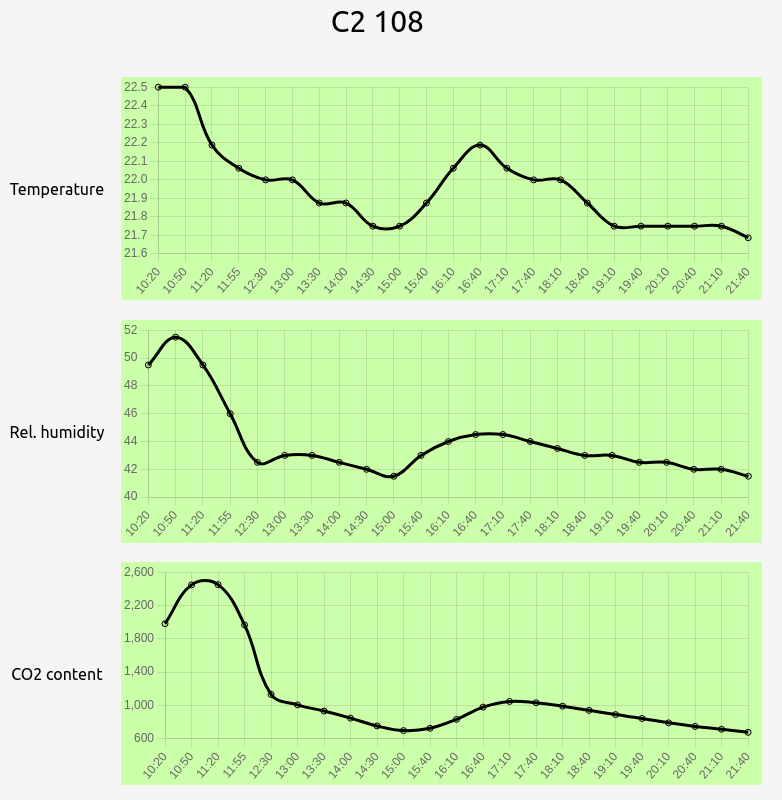
\includegraphics[width=\linewidth]{zdj/app/readings-c2108.png}
        \caption{Sala C2 108}
    \end{subfigure}
    \begin{subfigure}{0.5\textwidth}
        \centering
        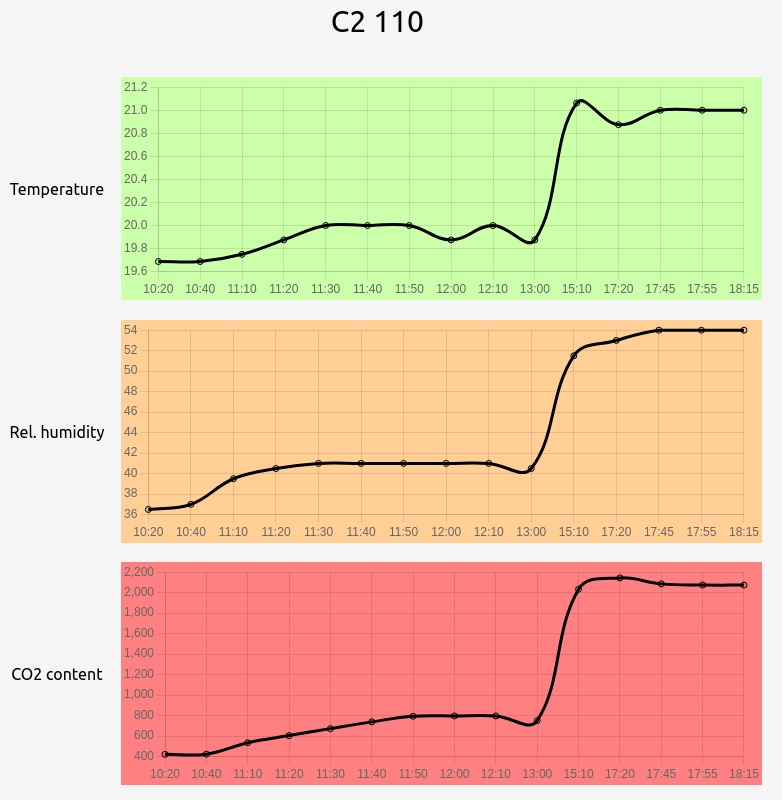
\includegraphics[width=\linewidth]{zdj/app/readings-c2110.png}
        \caption{Sala C2 110}
    \end{subfigure}
\end{figure}
\begin{figure}[H]
    \begin{subfigure}{0.5\textwidth}
        \centering
        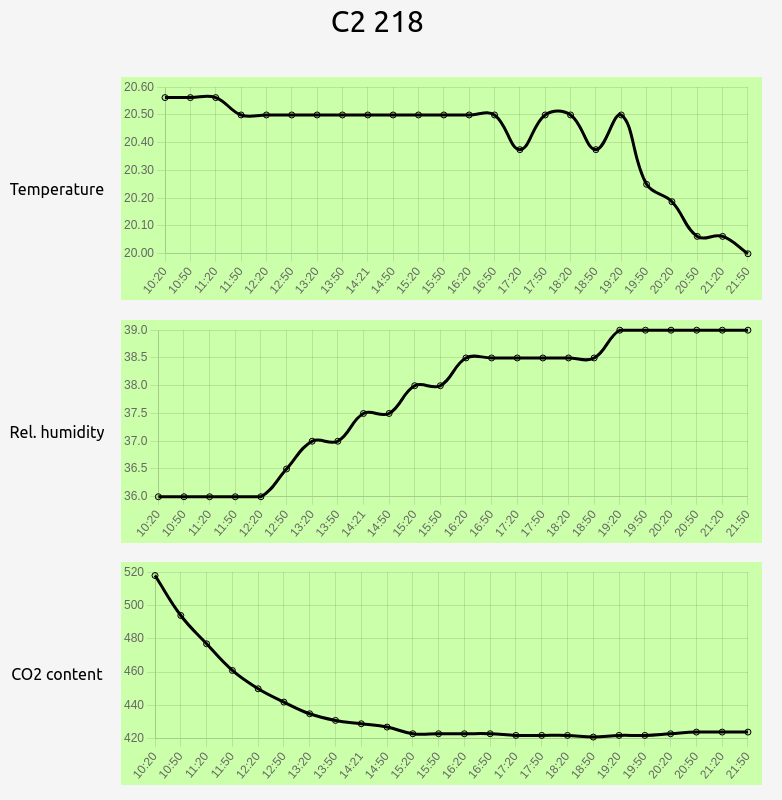
\includegraphics[width=\linewidth]{zdj/app/readings-c2218.png}
        \caption{Sala C2 218}
    \end{subfigure}
    \begin{subfigure}{0.5\textwidth}
        \centering
        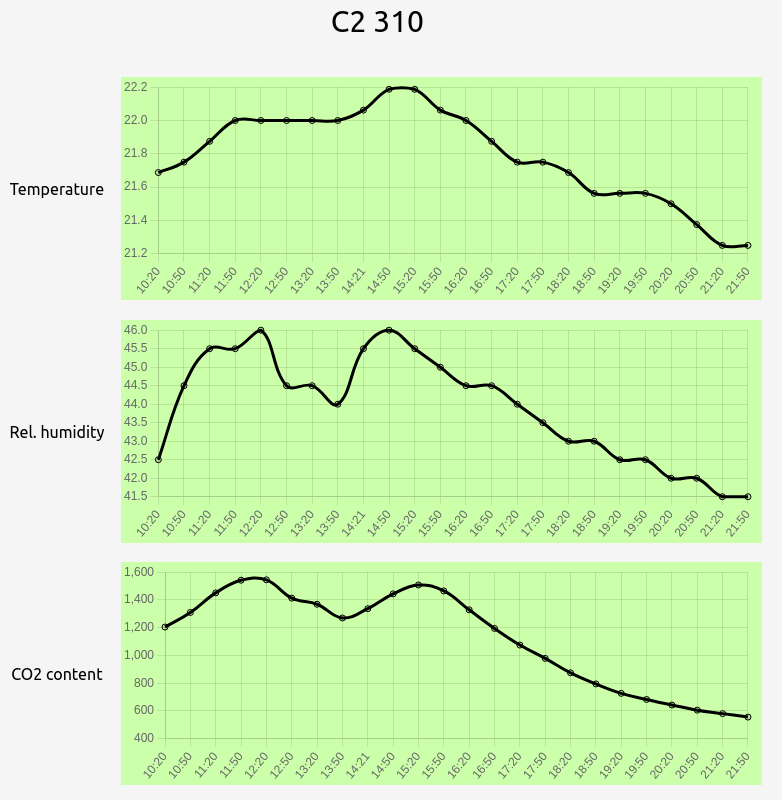
\includegraphics[width=\linewidth]{zdj/app/readings-c2310.png}
        \caption{Sala C2 310}
    \end{subfigure}
\end{figure}

Należy zaznaczyć, że w trakcie okresu zbierania odczytów czujnik z sali C2 110 często nie odpowiadał na zapytania 
o odesłanie danych sensorycznych. Z tąd też ostatni pomiar na wykresie jest z godziny 18:15 a nie z okolic godziny 
22:00, jak to ma miejsce w pozostałych salach.

W sali 108 pomiary wilgotności utrzymywały się w bezpiecznych przedziałach przez prawie cały
okres trwania badania, oprócz skoku około godziny 10:50. Temperatura zaś oscylowała wokół i często przekraczała
górną granicę optymalnego przedziału temperatur (18-22 st. C). Najgorzej dla tej sali prezentuje się stężenie dwutlenku węgla,
które w godzinach porannych znacznie przekraczało wskaźnik Pettenkofera.

Pomiary temperatury sali 110 natomiast wykazują się lepiej niż w sali 108, mieszcząc się w przedziale 18-22 z dużym
marginesem. Wilgotność pomimo gwałtownego skoku po godzinie 13:00 również była w normie przez większość dnia.
Najostrzejszą zmianą wykazuje się zaś stężenie CO2, które w ciągu dwóch godzin (13:00 - 15:10) zwielokrotniło
swoją wartość dwukrotnie. Na wszystkich trzech wykresach widać znaczący skok około godziny 13:00.

Najlepsze pomiary z pośród czterech sal wykazuje sala 218, w której wszystkie wartości pozostają w optymalnym
zakresie z dużym marginesem.

Wszystkie pomiary, oprócz stężenia CO2 pozostawały w normie dla sali 310. Widać jednak przekraczający wskazania
wzrost od godziny 10:20, który utrzymywał się do okolic godziny 18:00.

